\documentclass{article}
\usepackage{graphicx} % Required for inserting images
\usepackage{float}

\title{Albumes de Ye.}
\author{Diego Emiliano Sanchez Chavez}
\date{September 2026}

\begin{document}

\maketitle

\section*{Introducción}
Uno de mis artistas favoritos es Ye (anteriormente conocido como Kanye West), pues el, a pesar de estar envuelto en bastantes polemicas siempre, ha hecho tantas canciones que me encantan y me motivan. 

Por eso, en este documento hablaré un poco sobre los álbumes que más me gustan de toda su discorgrafía, y cuales son las canciones que más disfruto de el.
Creo que es imporante mencionar cuales son los albumes que ha hecho antes de comenzar con mis favoritos y las razones por las que me gustan.
\begin{itemize}
    \item \textbf{The College Dropout. (2004)}
    \item \textbf{Late Registration. (2005)}
    \item \textbf{Graduation. (2007)}
    \item \textbf{808's and Heartbreak. (2008)}
    \item \textbf{My Beautiful Dark Twisted Fantasy. (2010)}
    \item \textbf{Watch The Throne. (2011)}
    \item \textbf{Yeezus. (2013)}
    \item \textbf{The Life Of Pablo. (2016)}
    \item \textbf{Ye. (2018)}
    \item \textbf{Kids See Ghosts. (2018)}
    \item \textbf{Jesus Is King. (2019)}
    \item \textbf{Donda. (2021)}
    \item \textbf{Donda 2. (2022)}
    \item \textbf{Vultures. (2024)}
    \item \textbf{Vultures 2. (2024)}
    \item \textbf{Bully. (2026)}

    \end{itemize}
    
    Dicho esto, ahora si podemos comenzar con mis favoritos.
    \section*{The College Dropout}
    Este fue el primer albúm de estudio de Ye. Fue un toque completamente distinto al hiphop que existía en esos años, pues Ye hablaba de vulnerabilidad, criticas sociales, de la fé, etc, lo cual no tenía nada que ver con el rap que era popular en esos tiempos: el gangsta rap.
    Algo que me gusta mucho de Ye en general son los samples que utiliza en sus canciones, pues puede transofrmar canciones clásicas en canciones de hiphop y hacerlas sentir naturales.

    Entre todas las canciones que incluye este álbum, puedo destacar las siguientes:
    \begin{itemize}
    \item \textit{All Falls Down}: Habla sobre el consumismo, el materialismo (en especial el que afecta a la comunidad negra) y las inseguridades.
    \item \textit{Through The Wire}: Habla sobre el accidente que tuvo Ye al inició de su carrera, y como en vez de rendirse, siguió adeltante.
    \item \textit{Slow Jamz}: Habla sobre la nostalgia de las baladas de amor de los años 70s y 80s, y como las canciones de ahora ya no tienen ese romanticismo que solían tener las canciones antes.
    \item \textit{Family Business}: Probablemente una de mis favoritas de todos sus álbumes. Habla sobre el amor hacia la familia, la lealtad, y la nostalgia.
    \end{itemize}
    \begin{figure} [H]
        \centering
        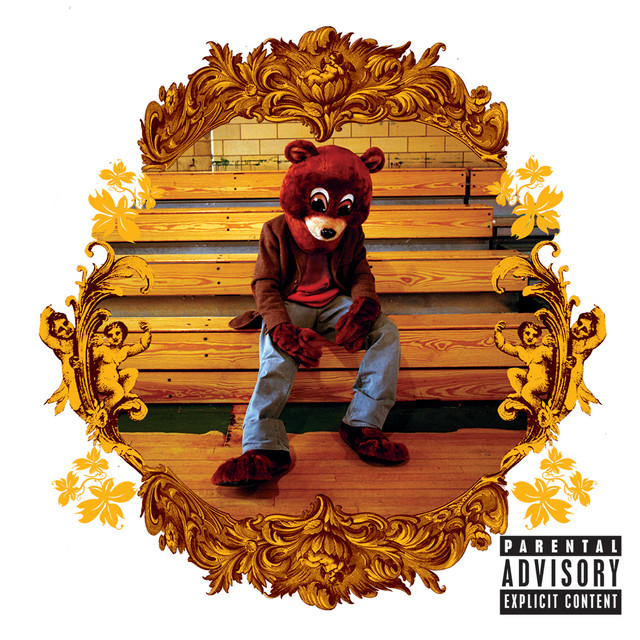
\includegraphics[width=0.75\linewidth]{image.png}
        \caption{Portada del álbum.}
    \end{figure}
    \section*{Graduation}
    Este sin duda es uno de sus albumes más famosos y más grandes. Se dice que el gangsta rap murió gracias a Graduation, pues el rapero 50Cent reto a a Ye, diciendole que si su álbum "\textit{Curtis}" vendía menos copias que Graduation el se retiraría. Y en efecto paso. Aunque 50 no se retiro, definitivamente marco un declive en el gangsta rap, e inspiro a más artistas a entrar al mundo del hiphop.
    Entre todas las canciones que conforman este álbum, estas son de mis favoritas:
    \begin{itemize}
        \item \textit{I Wonder}: Es otra de mis favoritas, está habla sobre la lucha para lograr tus sueños, sobre la identidad propia, y sobre la lucha para superar los obstaculos de la vida.
        \item \textit{Homecoming}: Habla acerca de la nostalgia que siente al volver a Chicago, la ciudad donde creció y de la que se tuvo que alejar para alcanzar la fama.
        \item \textit{Big Brother}: Es una canción dedicada a Jay-Z, su mentor, en donde expresa su admiración y gratitud hacia el.
        \item \textit{Bittersweet Poetry}: Es otra de mis canciones favoritas de el. Es una canción exclusiva para la región japonesa, pero se encuentra en YouTube. En pocas palabras, relata una relación tóxica y destructiva, donde siente que no quiere a su pareja pero a la vez siente que la necesita.
        
    \end{itemize}
    \begin{figure} [H]
        \centering
        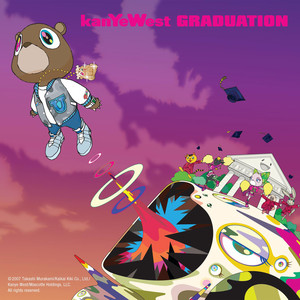
\includegraphics[width=0.75\linewidth]{image2.png}
        \caption{Portada del álbum}
    \end{figure}
    \section*{Yeezus.}
    Este álbum se cararactrizo por sus sonidos industriales y que estaban fuera de lo ordinario. Igualmente se caracterizo por el ego que maneja en varias de las canciones.

    Entre mis favoritas se encuentran: 
    \begin{itemize}
        \item \textit{On Sight}: Es la canción inicial del álbum. En esta, desafía a la crítica y la industria musical, y se puede notar desde los sonidos que utiliza desde el comienzo hasta el final de la canción.
        \item \textit{I Am A God}: En esta canción, como bien lo dice el nombre, Ye se toma a si mismo como una deidad de la industria musical. Igualmente aborda temas como la rebelión contra las corporaciones, etc.
        \item \textit{Black Skinhead}: Es una canción que aborda temas de racismo, de protesta y de resistencia al sistema.
        \item \textit{New Slaves}: En esta canción, Ye nos dice que la esclevitud no desapareció, si no que evoluciono a la esclavitud mental que se ha impuesto por el capitalismo.
        \item \textit{Bound 2}: Es una canción dedicada a su ahora ex-esposa Kim Kardashian, sobre su amor imperfecto y caótico.
    \end{itemize}
    \begin{figure} [H]
        \centering
        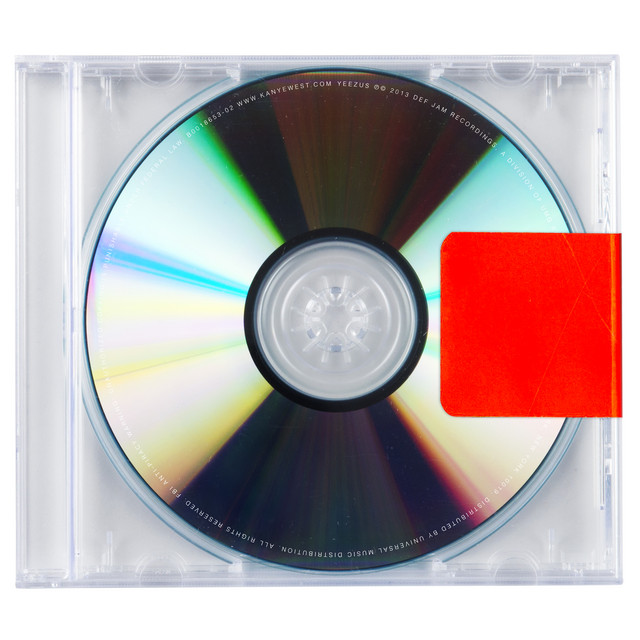
\includegraphics[width=0.70\linewidth]{image3.png}
        \caption{Portada del álbum}
    \end{figure}
    \section*{The Life Of Pablo}
    Este álbum hace referencia a tres Pablos, y como Ye relaciona la vida de cada uno con la suya. Pablo Escobar, Pablo Picasso, y San Pablo. ES un álbum que habla acerca de la vida religiosa y la vida de éxito. Es un álbum bastante extenso, pero estas son mis canciones favoritas:
    \begin{itemize}
        \item \textit{Ultralight Beam}: Es la canción inicial del álbum. Habla sobre la fé, la redención, y busqueda de paz.
        \item \textit{Father Stretch My Hands Pt.1}: Habla explicitamente de una modelo, de las relaciones casuales, y el miedo de perder a su familia. Básicamente, la contradicción que se nos presenta en la portada del álbum.
        \item \textit{Famous}: Habla sobre el costo que tiene la fama, la provación mediatica, y el ego. En esta canción, Ye se declara culpable de haber hecho famosa a Taylor Swift.
        \item \textit{No More Parties In L.A}: En esta canción, Kandrick Lamar y Ye pintan a la ciudad como un lugar lleno de relaciones por interés, infidelidades, fiestas vacias, adicciones a las redes, etc. 
        
    \end{itemize}
    \begin{figure} [H]
        \centering
        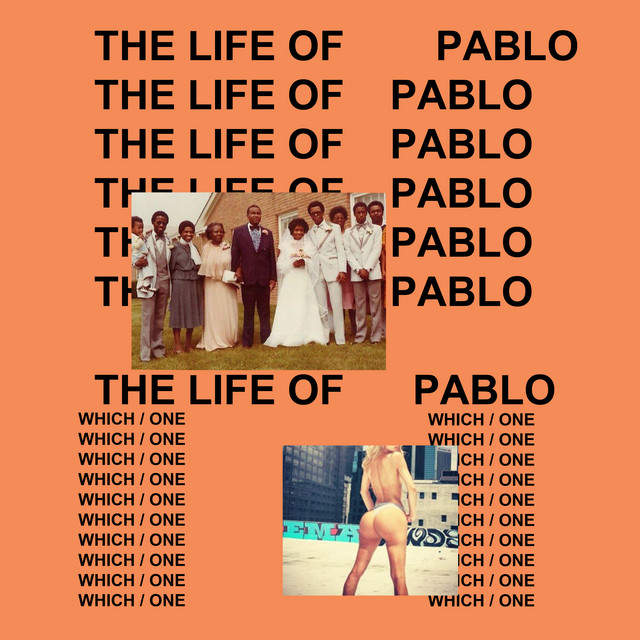
\includegraphics[width=0.75\linewidth]{IMAGE.png}
        \caption{Portada del álbum.}
    \end{figure}
    \section*{Conclusión}
    En general, esos cuatro son de mis álbumes favoritos de Ye, aunque definitivamente disfruto todos, ya que cada uno tiene su toque y su estilo diferente, así como una canción que me guste. Pero considero yo que estos cuatro albumes tienen las mejores temáticas y las mejores canciones de toda su discografía.
\end{document}
